%Autor: Piotr Woźniak
% !TeX program = xelatex
\documentclass[12pt, twoside, openany]{mwrep}
\usepackage{polski}
\usepackage[T1]{fontenc}
\usepackage[utf8]{inputenc}
\usepackage{graphicx}
\usepackage[a4paper,top=25mm,bottom=25mm,left=30mm,right=20mm,bindingoffset=0mm]{geometry}
\usepackage{blindtext}
\usepackage{helvet}
\usepackage{fancyhdr}
\usepackage{fontspec}
\usepackage{enumerate}
\usepackage{amssymb}
\usepackage{amsmath}
\usepackage{mathrsfs}
\usepackage[usenames, dvipsnames]{color}
\usepackage{gensymb}
\usepackage{float}
\usepackage{cite}
\usepackage[chapter]{algorithm}
\usepackage{mleftright}
\usepackage[noend]{algpseudocode}
\usepackage{lipsum}

\newcommand{\lnn}[1]{%
  \ln\left(#1\right)%
}

\newcommand{\lnb}[1]{%
  \ln\mleft(#1\mright)%
}

\floatname{algorithm}{Algorytm}

\renewcommand{\algorithmicrequire}{\textbf{Na wejściu:}}
\renewcommand{\algorithmicensure}{\textbf{Na wyjściu:}}
\renewcommand{\algorithmicprocedure}{\textbf{funkcja}}

\renewcommand{\listalgorithmname}{Spis algorytmów}

\DeclareMathOperator{\sign}{sign}

%%%%%czcionki
\setromanfont[
BoldFont=timesbd.ttf,
ItalicFont=timesi.ttf,
BoldItalicFont=timesbi.ttf,
]{times.ttf}

\setsansfont[
BoldFont=arialbd.ttf,
ItalicFont=ariali.ttf,
BoldItalicFont=arialbi.ttf
]{arial.ttf}
%%%%%

\linespread{1.15}
\setlength{\parindent}{0.5cm}

\pagestyle{fancy}
\fancyhead{}
\renewcommand{\chaptermark}[1]{\markboth{\thechapter.\ #1}{}}
\fancyhead[RO]{\nouppercase{\leftmark}}
\fancyhead[LE]{\nouppercase{\rightmark}}
\renewcommand{\headrulewidth}{0.4pt}
\fancyfoot{}
\fancyfoot[LE,RO]{\thepage}

\fancypagestyle{opening}{%
  \fancyhf{}\fancyfoot[LE,RO]{\thepage}%
  \renewcommand{\headrulewidth}{0pt}}
  
\fancypagestyle{closing}{%
  \fancyhf{}\fancyhead[RO]{\nouppercase{\leftmark}}\fancyhead[LE]{\nouppercase{\rightmark}}\fancyfoot[LE,RO]{\thepage}%
  \renewcommand{\headrulewidth}{0.4pt}}
  

\newtheorem{theorem}{Twierdzenie}[section]

\begin{document}

%--------------------------------------------------------------
%Strona tytułowa
\begin{titlepage}
    \begin{center}
        %{\fontfamily{phv}\selectfont
        {\sffamily
            \begin{center}
                
\includegraphics[width=\textwidth]{titlepage/szablonEITI.png}\\   
            \end{center}
            \hfill \break
            \hfill \break
            Instytut XXXXXX\\
            \hfill \break
            \hfill \break
            \begin{center}
                
\includegraphics[width=\textwidth]{titlepage/szablonMGR.png}\\
            \end{center}
            na~kierunku XXXXX\\
            w~specjalności XXXXX\\
            \hfill \break
            \hfill \break
            \large
            Tytuł\\
            \hfill \break
            \hfill \break
            \LARGE
            Xxxx Xxxx\\
            \normalsize
            Numer albumu xxxxxx\\
            \hfill \break
            \hfill \break
            promotor\\
            prof. dr~hab. inż. Xxx Xxx\\
            \vfill
            WARSZAWA 2019
        }
    \end{center}
    \newpage
    \thispagestyle{empty}
    \hfill
    
    \newpage

\end{titlepage}
%-----------------------------------------------------------------------------------------

\thispagestyle{empty}
\newpage
\hyphenation{Syl-ves-tra}
\hyphenation{Syl-ves-ter-a}

\newpage
\setcounter{page}{1}

%------------------------------------------------------------------------------
%Streszczenie PL
\thispagestyle{empty}
\centerline{\bf Streszczenie}
\centerline{\bf Tytuł}
\noindent\textit{\lipsum[1-4]}\\
\\
\textbf{Słowa kluczowe:} xxx
\clearpage

%------------------------------------------------------------------------------
%------------------------------------------------------------------------------
%Streszczenie ENG
\thispagestyle{empty}
\centerline{\bf Abstract}
\centerline{\bf Title}
\noindent\textit{\lipsum[1-4]}\\
\\
\textbf{Keywords:} xxx
%------------------------------------------------------------------------------
\newpage
\thispagestyle{empty}
\begin{figure}[H]
\vspace{-55pt}%
\noindent\makebox[\textwidth]{%
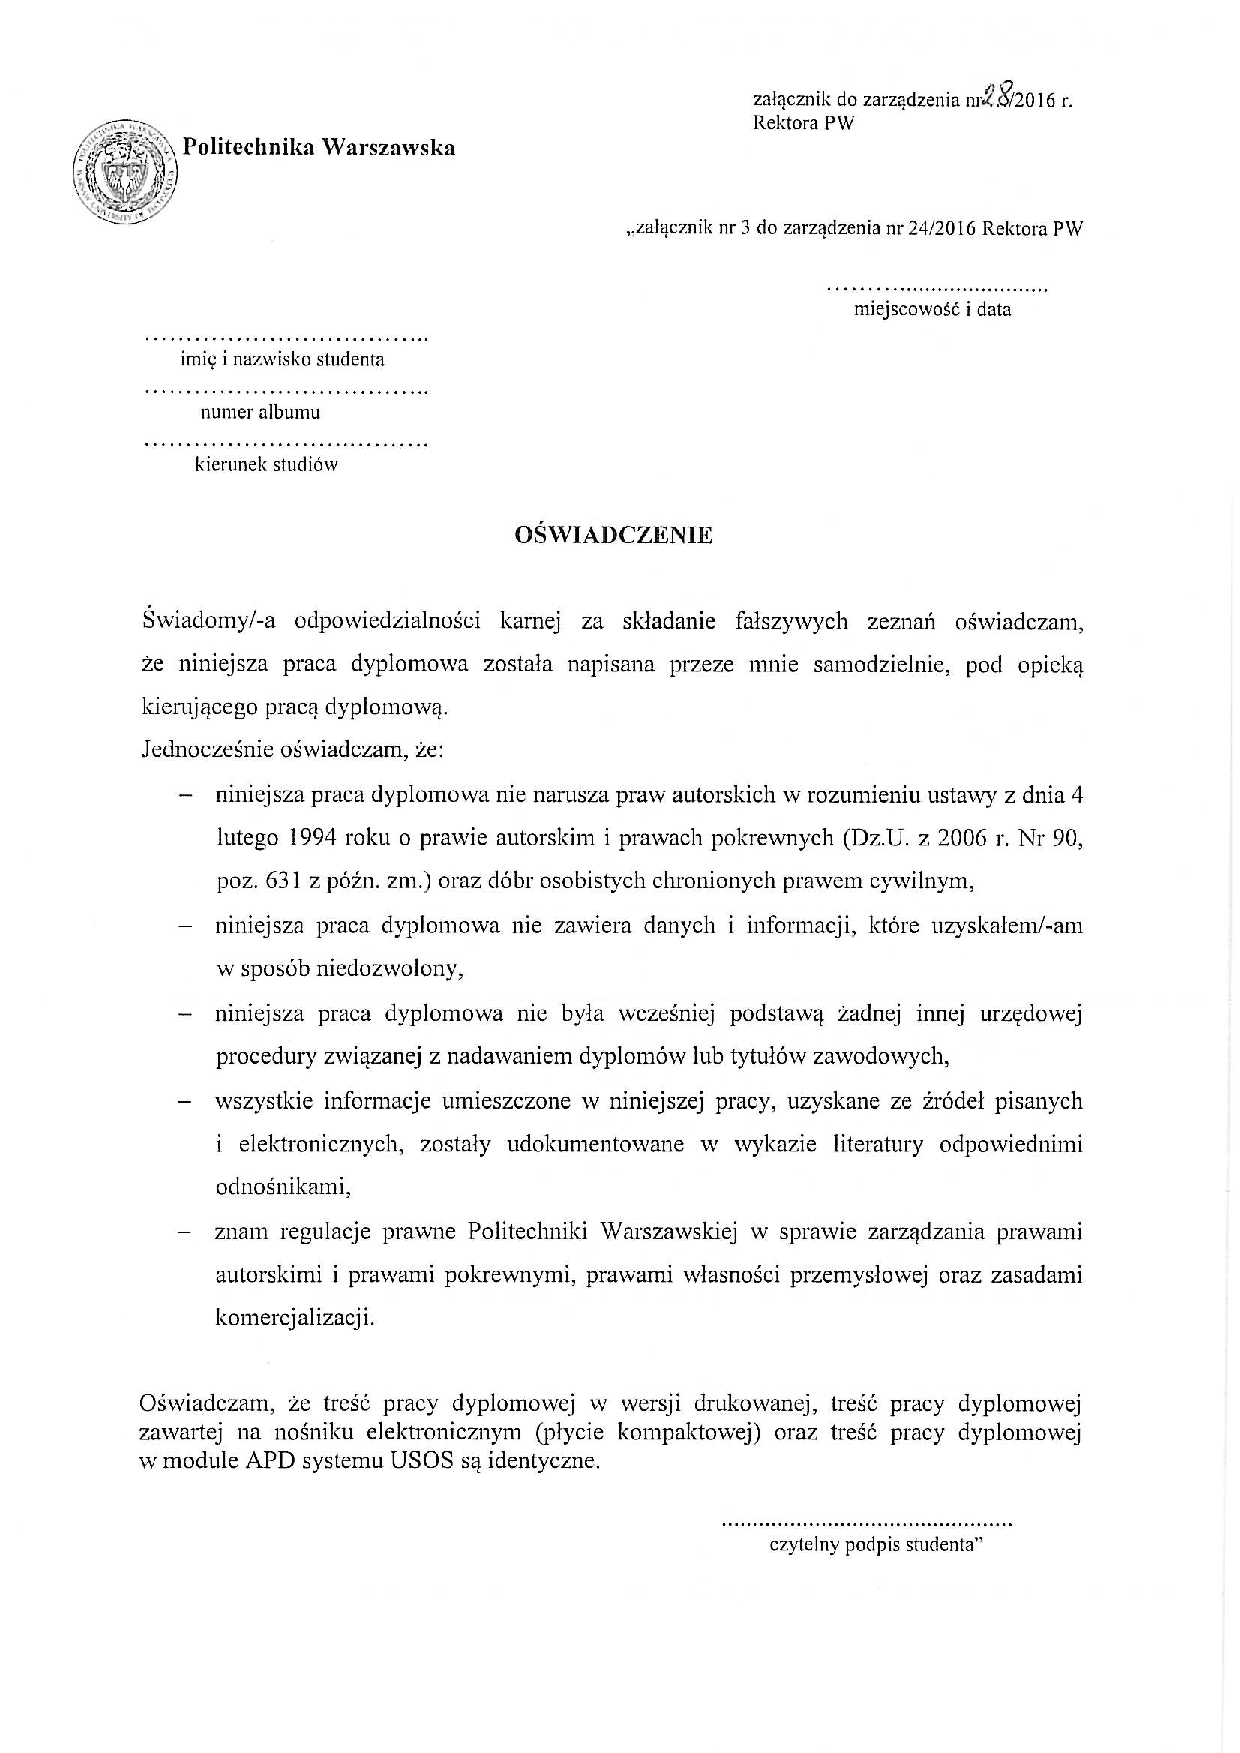
\includegraphics[width=1.3\textwidth]{./pdfs/2strona.pdf}}
\end{figure}
\newpage

%Spis treści
\tableofcontents
\clearpage

%------------------------------------------------------------------------------
%----POCZĄTEK----
\chapter{Wstęp}
\lipsum[1-4]
\section{Sekcja 1.}
\lipsum[1-10]

\chapter{Rozdział 1.}
\lipsum[1-4]
\section{Sekcja 1.}
\lipsum[1-10]

%----KONIEC------------------------

\begin{thebibliography}{99}
\bibitem[1]{MotionBlur} Aizenberg, Igor, et al. Blur identification by multilayer neural network based on multivalued neurons. IEEE Transactions on Neural Networks, 2008, 19(5), s. 883-898.

\end{thebibliography}

\listoffigures

\listoftables

\listofalgorithms

%----Bibliografia------------------

\end{document}

